% !TeX root = bash.tex
\section{II. CLI}
\begin{frame}
\frametitle{The CLI}
\textbf{CLI} stands for \textbf{command line interface}, as opposed to a GUI.

\begin{figure}[h]
    \centering
    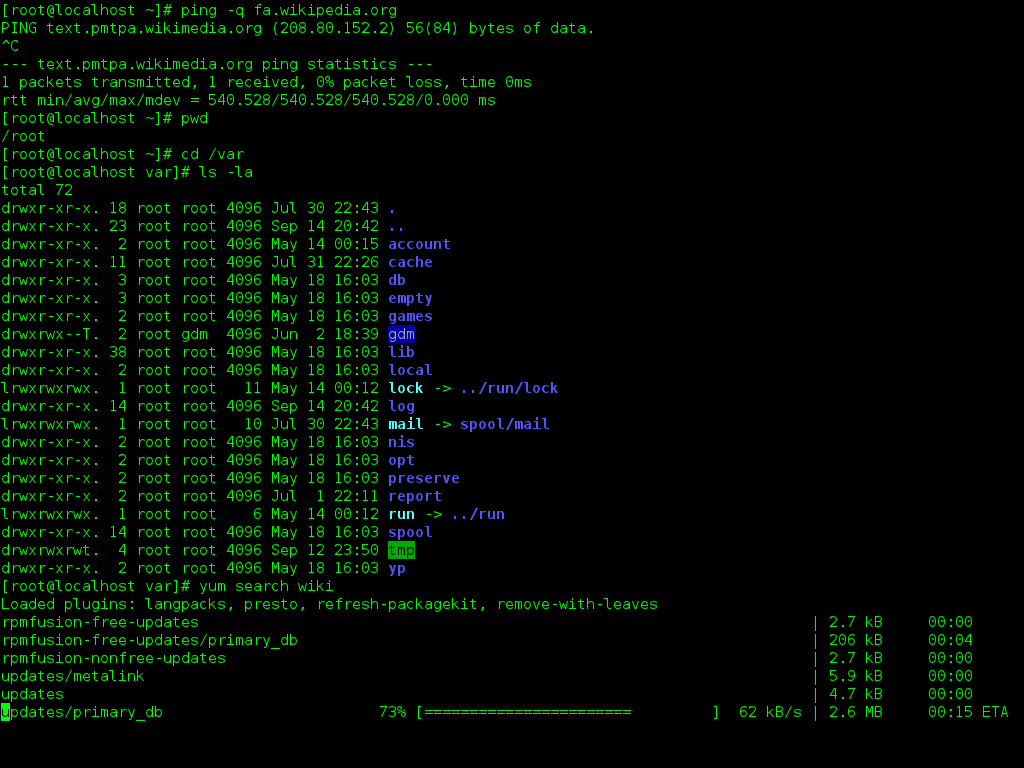
\includegraphics[height=5cm]{cli}
    \caption{A stereotypical, Hollywood-like CLI.}
\end{figure}
\end{frame}

\begin{frame}[fragile]
\frametitle{Anatomy of a command (part 1)}
\begin{lstlisting}[language=bash]
# get first 5 lines of file
$ head -n 5 longfile.txt
\end{lstlisting}
\begin{tabular}{ll}
    \tt{head}            & Executable file somewhere \\
    \tt{-n}                & Option (aka flag) \\
    \tt{5}                & Argument to \tt{-n} \\
    \tt{longfile.txt}    & Argument to \tt{head}
\end{tabular}
\end{frame}

\begin{frame}[fragile]
\frametitle{Anatomy of a command (part 2)}
Anatomy of a command:
\begin{lstlisting}[language=bash]
# list all files but *.o recursively in reverse
$ ls -Rr --ignore='*.o'
\end{lstlisting}
\begin{tabular}{ll}
    \tt{ls}            & Executable in \tt{\$PATH} \\
    \tt{-Rr}        & Two options: \tt{-R -r} \\
    \tt{--ignore=}    & Long option \\
    \tt{'*.o'}        & Argument to \tt{--ignore}
\end{tabular}
\begin{block}{Notes}
    \begin{itemize}
        \item Not every program uses this \tt{--long-option} convention
        \item The equal sign after \tt{--ignore} is optional in this command
        \item \tt{'*.o'} does \textit{not} expand to a list of files.
            It is simply a string.
    \end{itemize}
\end{block}
\end{frame}

\begin{frame}[fragile]
\frametitle{I can't possibly remember all \tt{--this} and \tt{--that}!}
You don't need to, thanks to \textbf{man pages}! (Short for manual pages)

Try:
\begin{lstlisting}[language=bash]
$ man ls
\end{lstlisting}

If it doesn't work, try \url{https://man.archlinux.org/man/ls.1}
\end{frame}

\begin{frame}[fragile]
\frametitle{Challenge}
\begin{itemize}
    \item Read the man page for \tt{head}
    \item Experiment with files in \tt{02-cli/}
    \item Find a command to generate the following:
\end{itemize}
\begin{lstlisting}[language=bash]
==> p0.txt <==
MANIFESTO OF THE COMMUNIST PARTY.

==> p1.txt <==
I. BOURGEOIS AND PROLETARIANS.
\end{lstlisting}
\end{frame}

\begin{frame}[fragile]
\frametitle{Learning by doing}
Inside \tt{02-cli/}, run:
\begin{lstlisting}[language=bash]
$ diff sway.1.conf sway.2.conf
\end{lstlisting}
Congratulations, you just learned how to use \tt{diff}!
\newline \newline
\begin{lstlisting}[language=bash]
$ diff sway.1.conf sway.2.conf
\end{lstlisting}
\end{frame}

\begin{frame}
\frametitle{Lifehacks\footnote{Should work in most shells.}}
\begin{itemize}
    \item Use $\uparrow \downarrow$
    \item \tt{Ctrl-W}: delete one word to the left
    \item \tt{Ctrl-U}: delete everything to the left
    \item \tt{Ctrl-K}: delete everything to the right
    \item \tt{Ctrl-7}: undo
    \item \tt{Ctrl-C}: abort
    \item \tt{Ctrl-R}: search history
\end{itemize}
\end{frame}

